% Contributors: Alexandre Lamy, Trung Vu
\section{The motivation for density-based clustering}
  \subsection{The problem with centroid-based clustering}

To motivate density-based clustering, we have to understand the
shortcomings of centroid-based clustering. The first is that it makes
some strong assumptions on what a cluster should look like. Consider the following data set
in $\mathbb{R}^2$.

\begin{center}
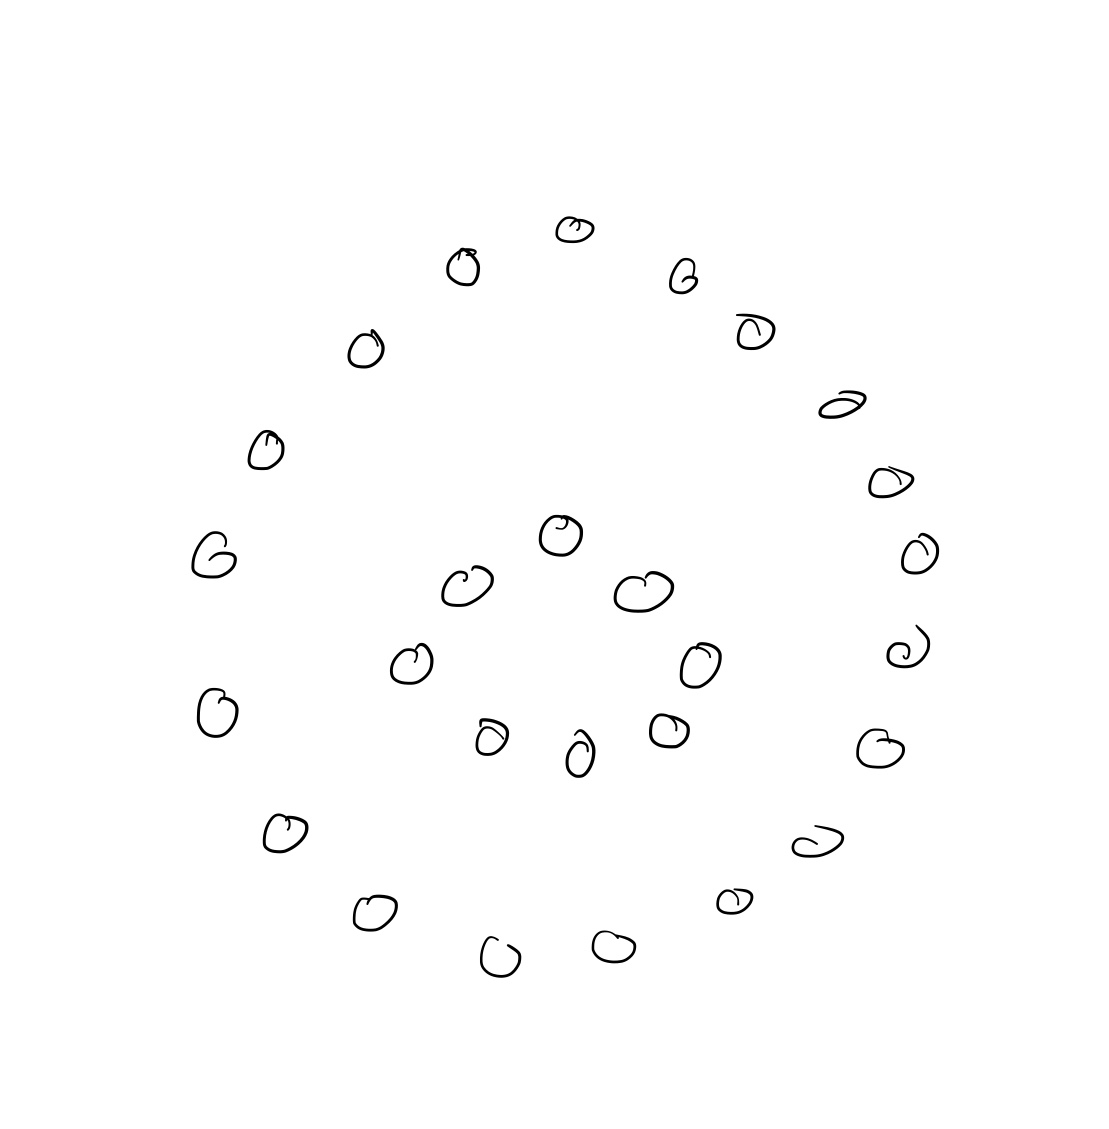
\includegraphics[width=.7\linewidth]{chapter_2/images/raw.jpg}
\end{center}

Our intuition suggests that each concentric circle should form its own cluster.
Thus the "ideal" clustering, according to our intuition, should look something
like this:

\begin{center}
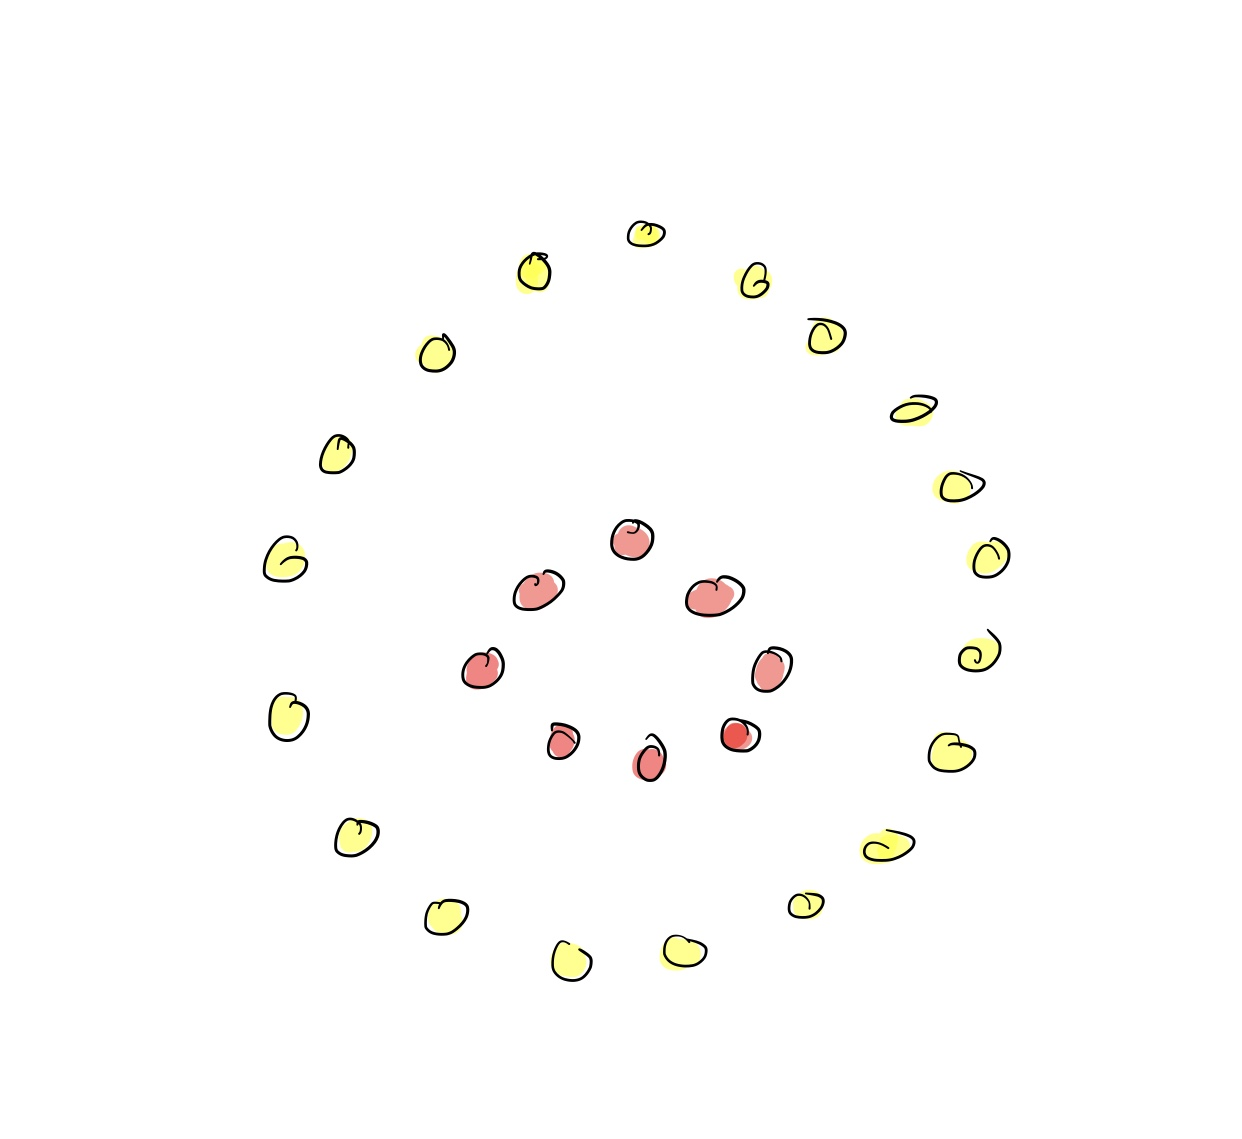
\includegraphics[width=.7\linewidth]{chapter_2/images/intuition.jpg}
\end{center}

However, running $k$-means on this dataset produces the following clustering.

\begin{center}
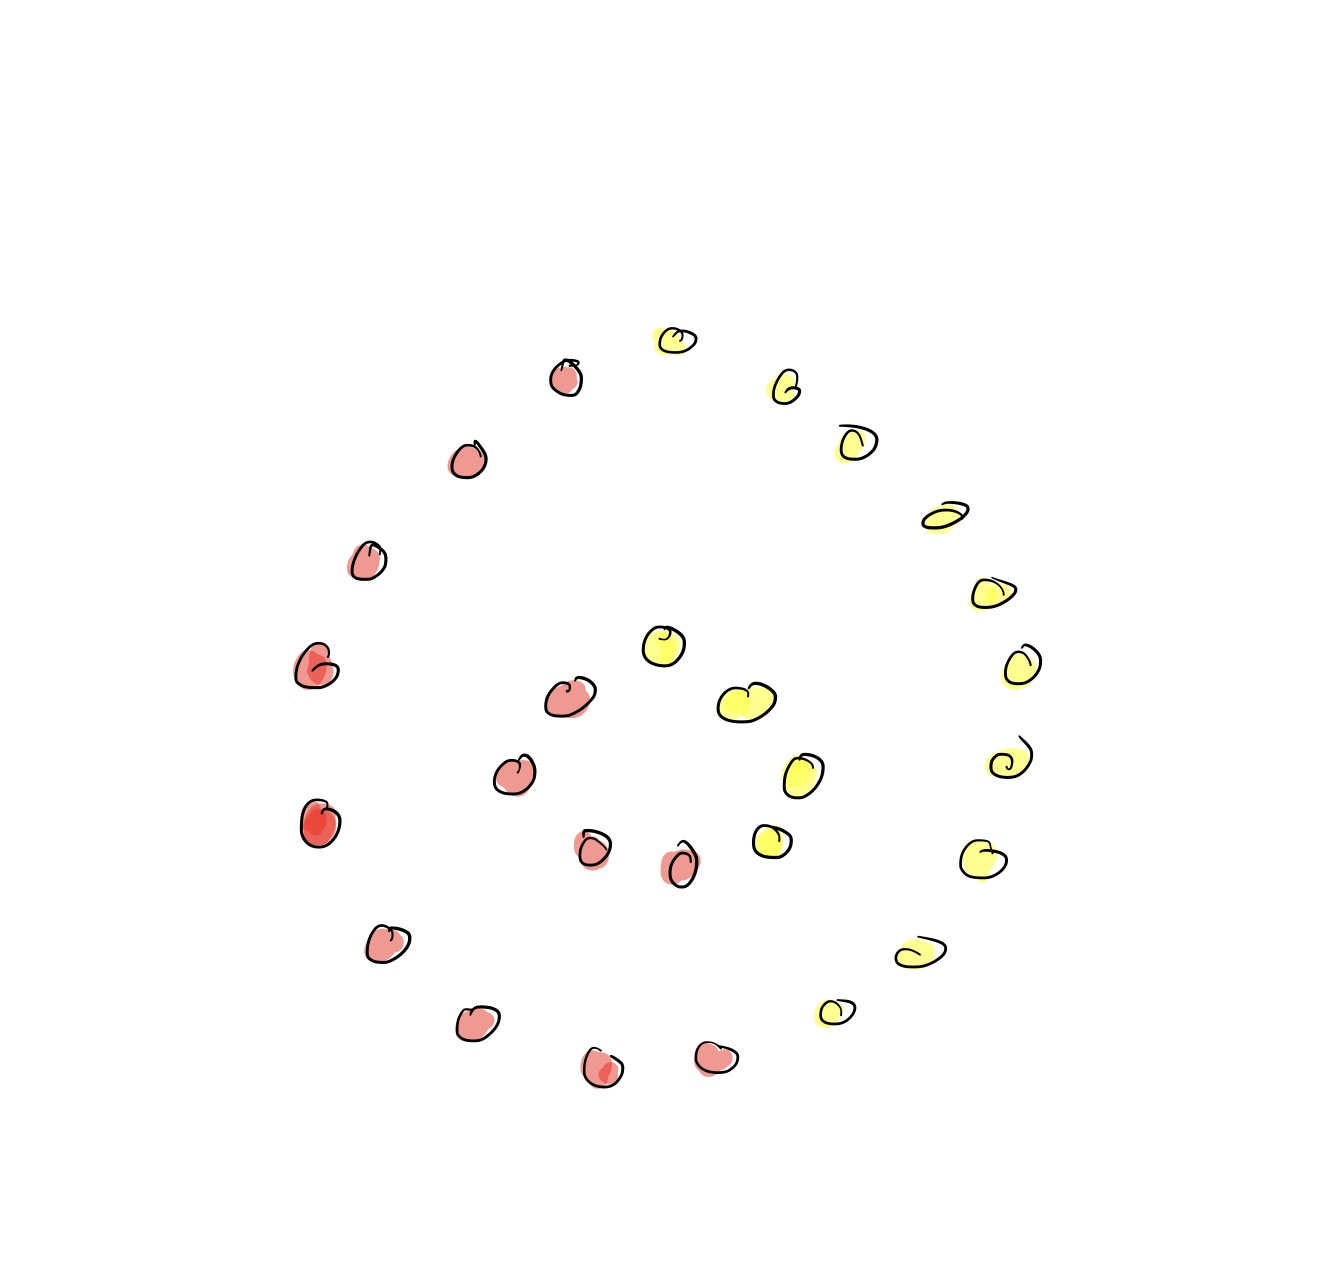
\includegraphics[width=.7\linewidth]{chapter_2/images/kmeans.jpg}
\end{center}

Why is it the case that $k$-means fails to comply to our intuition in the example
above? The answer is the convexity of the partitions generated by centroids. Roughly,
if you draw a line between any given points in a partition then all the points
between those two points should also be in that partition. Thus the reason
why the partition found by $k$-means looks like this:

\begin{center}
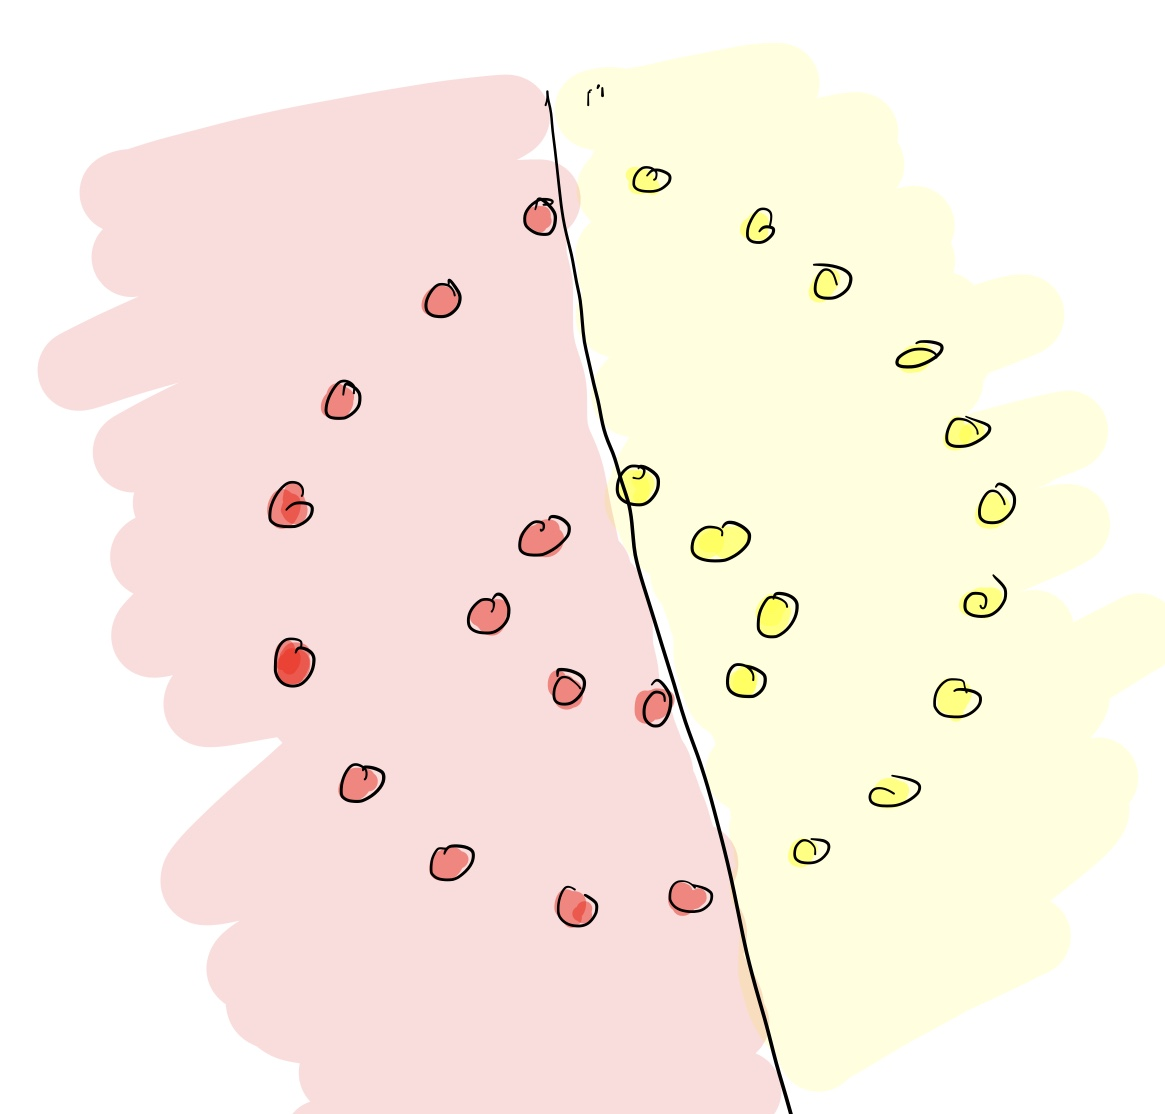
\includegraphics[width=.7\linewidth]{chapter_2/images/voronoi-cell.jpg}
\end{center}

The partitions induced by centroids are called Voronoi cells: the Voronoi
cell of a point $x$ of a metric space $\mathcal{X}$ is the set of points
$y$ whose distance to $x$ is not greater than any other points $x' \in \mathcal{X}$.
Each partition of $k$-means is a Voronoi cell of a centroid. It is a fact that
Voronoi cells are convex.

However, convexity is not always what we're looking for in a partition. Our intuition
roughly partitions the space up like this:

\begin{center}
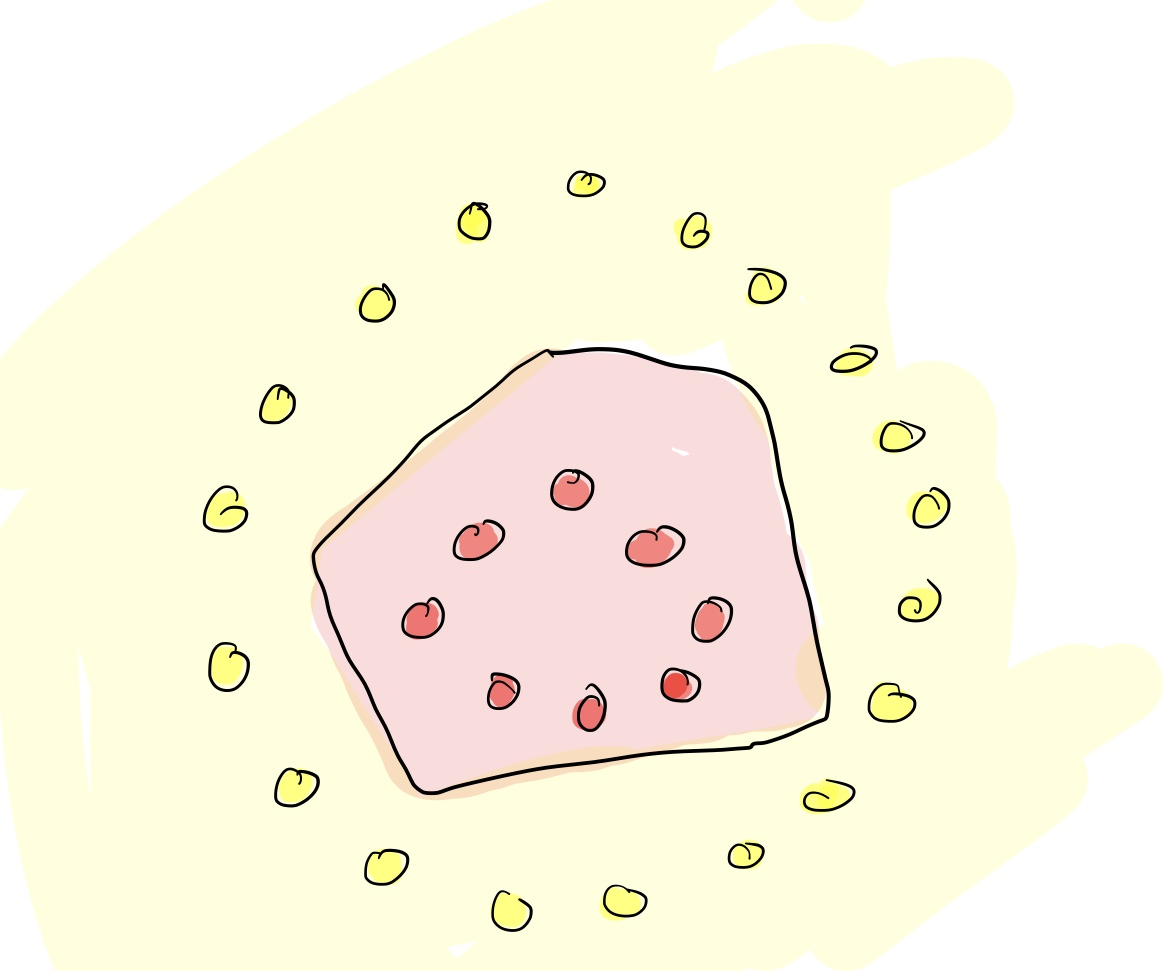
\includegraphics[width=.7\linewidth]{chapter_2/images/intuition-cell.jpg}
\end{center}

If you draw a line between any two yellow points then that line will
cross the red section. This implies that the yellow partition is not a convex
set. Thus this partition is not achievable by $k$-means. As we will see
in the next section, density-based clustering can address this shortcoming.

The second drawback of centroid-based clustering methods is that we have
to specify the number of clusters we want. This can be quite difficult. Given
a dataset of more than 3 dimension, how do we even know what number of clusters
we want if we can't even visualize the data?

\subsection{The intuition behind density-based clustering}

The intuition behind density-based clustering is that "dense" regions of data
that are close together should be in the same cluster. To make an analogy,
the high-density regions, which are clusters in density-based clustering, are the continents,
while the low-density regions is the ocean that surround and separate these
continents.

Since the high-density regions are not convex, we have escaped the curse of
convexity! Furthermore, since we are simply following the density of the data,
we do not have to specify the number of clusters before hand. We will see the
details in the next section.
